\chapter{Introduction}\label{ch:introduction}

This is a technical research paper covering the scientific part of the development 
of the open-source MoleHole project\footnote{\url{https://github.com/g-martin772/MoleHole}}. 
It is not a user manual, neither a tutorial, and it is not particularly intended to be read linearly.
This paper aims to cover both the very foundational concepts of computer graphics, physics and mathematics,
as well as highly specific technical details about general relativistic ray tracing and physical simulations.
The reader is encouraged to read the table of contents first and jump between sections of interest.

\section{Motivation}\label{sec:motivation}

Inspired by the visual display of the black hole \emph{Gargantua} in the movie \emph{Interstellar}\cite{Nolan2014Interstellar},
and a general interest in computer graphics and physics, we decided to build a black hole simulator.
What started as a simple school project soon evolved into a more ambitious project,
aiming to create an interactive application able to export physically accurate renderings
of black holes and other stellar objects.

For \emph{Interstellar}, the visual effects company ``Double Negative'' developed the \gls{dngr},
which traces bundles of light rays through the spacetime of a spinning black hole instead individual ones\cite{James15}.
The spin was lowered from $a/M = 0.999$ to $a/M = 0.6$ 
because the flattened shadow edge and multiple disk images
were deemed too confusing for a general audience\cite{James15}.
The same code was later used for scientific publications.
For example the visualization of the movie's wormhole\cite{James15b}.

In 2019 the \gls{eht}, 
a global network of radio telescopes combined through \gls{vlbi} at a wavelength of \SI{1.3}{\milli\metre},
published the first image of the supermassive black hole M87*\cite{EHT19}.
In 2022 the image of Sagittarius~A*, the black hole at the center of the Milky Way Galaxy\cite{EHT22}.
\Cref{fig:motivation-images} shows these images next to the \gls{dngr} rendering.

\begin{figure*}[t]
    \centering
    \begin{subfigure}[t]{0.49\textwidth}
        \centering
        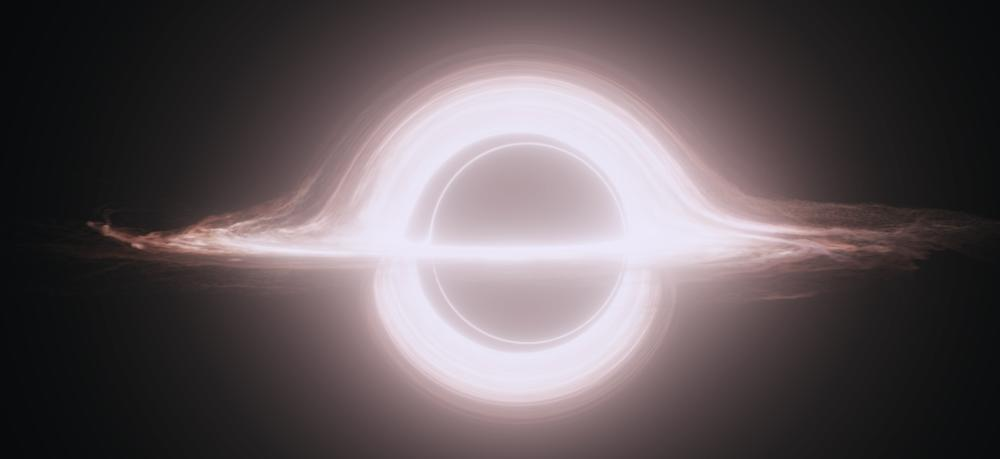
\includegraphics[height=3.6cm]{intro/gargantua-dngr.jpg}
        \caption{\emph{Interstellar} (\gls{dngr}), $a/M = 0.6$}
    \end{subfigure}\hfill
    \begin{subfigure}[t]{0.27\textwidth}
        \centering
        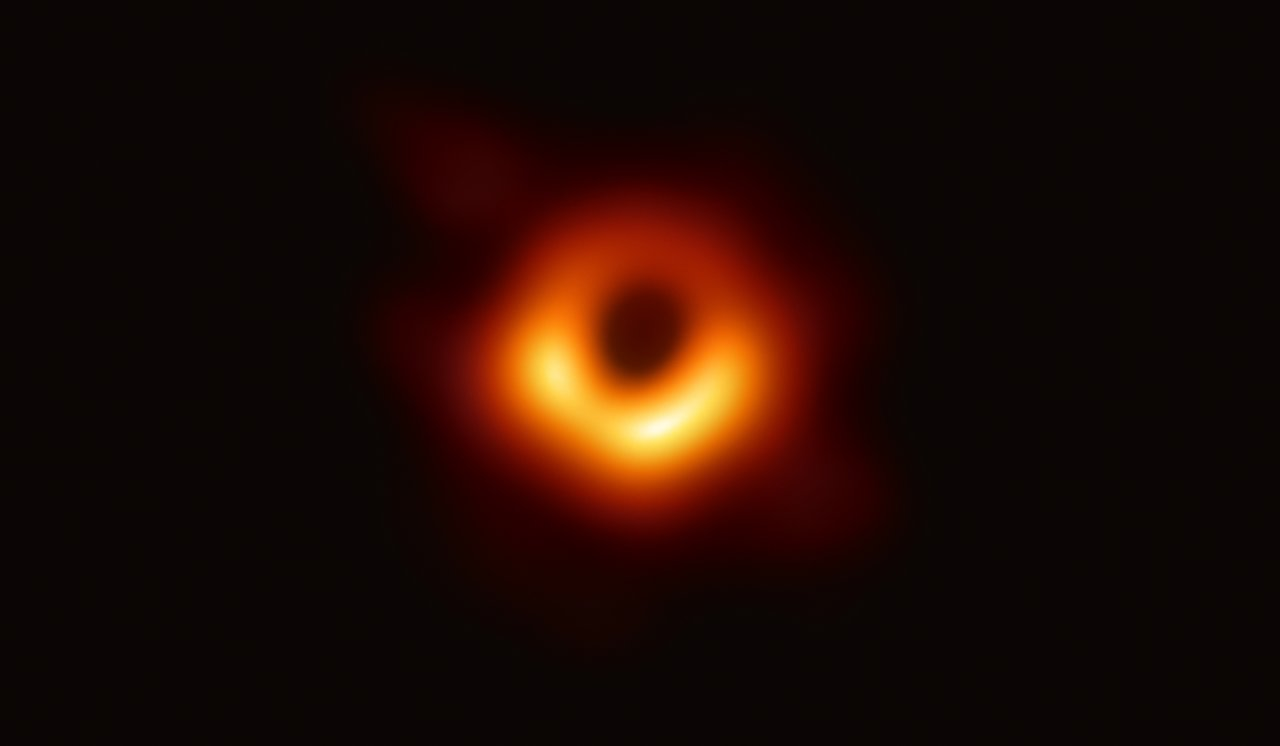
\includegraphics[height=3.6cm, trim=300 66 300 60, clip]{intro/m87-eht-2019.jpg}
        \caption{M87*, \gls{eht} 2017}
    \end{subfigure}\hfill
    \begin{subfigure}[t]{0.23\textwidth}
        \centering
        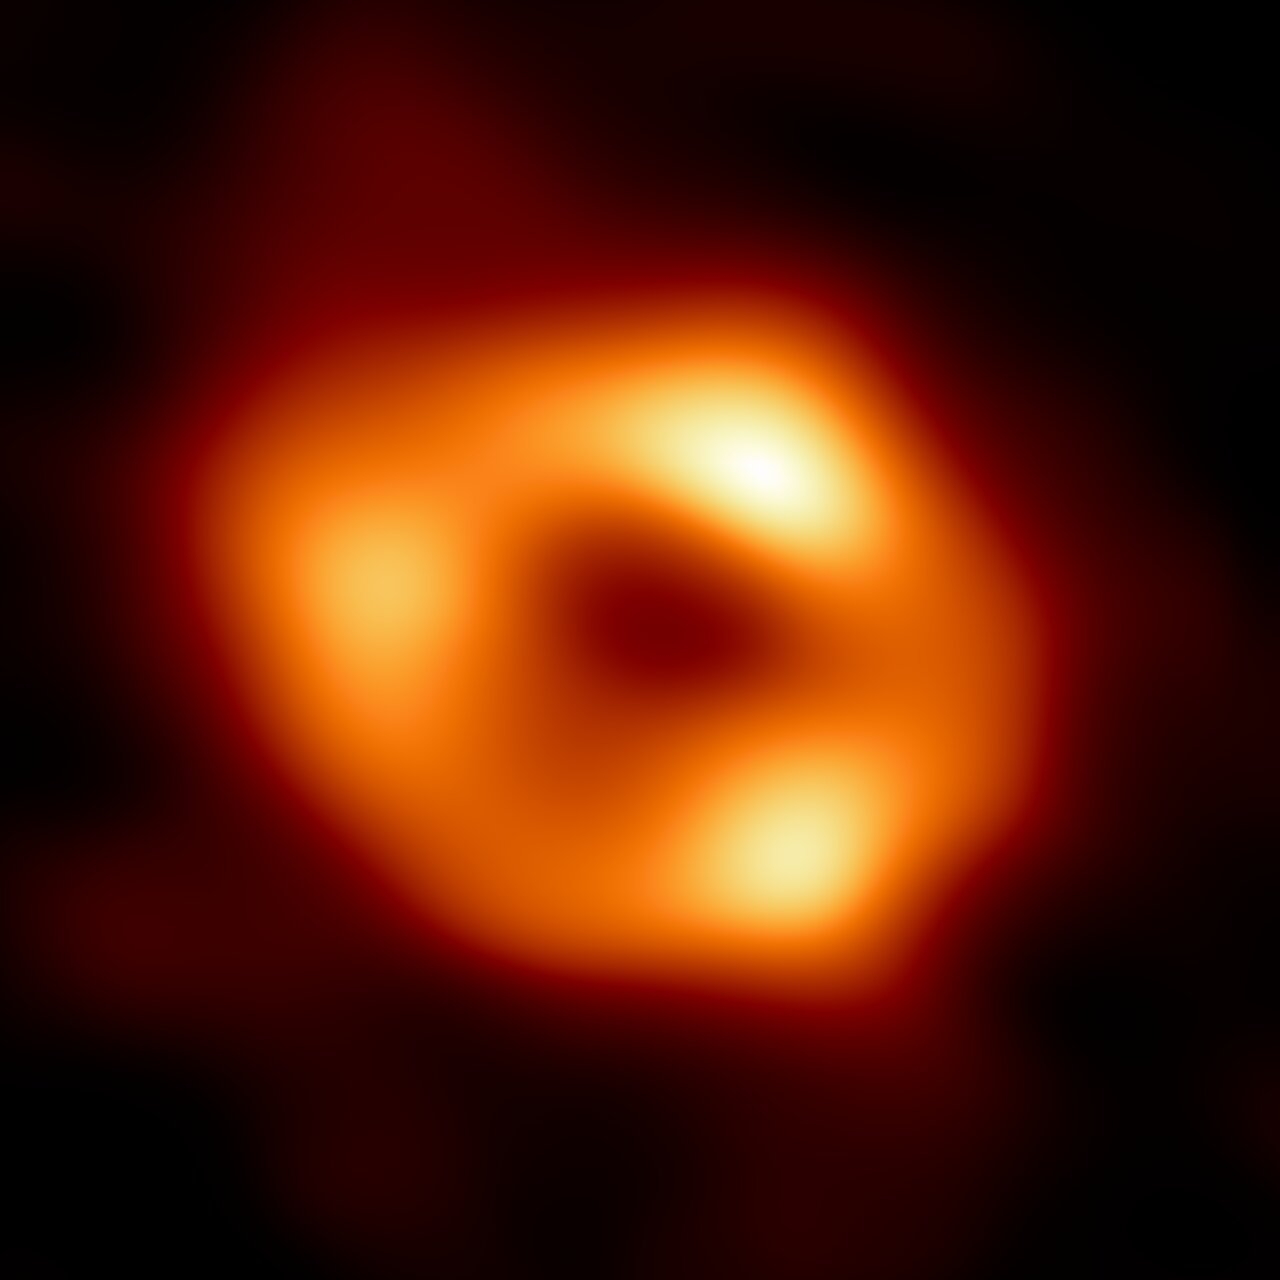
\includegraphics[height=3.6cm]{intro/sgra-eht-2022.jpg}
        \caption{Sgr~A*, \gls{eht} 2022}
    \end{subfigure}
    \caption{A simulated and two observed black hole images.
    (a)~Rendered with \gls{dngr}. A variant of the disk seen in \emph{Interstellar}\cite{James15}.
    (b)~M87*\cite{EHT19}
    (c)~Sagittarius~A*\cite{EHT22}
    \label{fig:motivation-images}}
\end{figure*}


\section{Related Work}\label{sec:related-work}
\planned{DNGR, GYOTO, GRay, RAPTOR, geokerr, GeodesicViewer, Riazuelo}

\section{Problem Statement and Contributions}\label{sec:problem-statement-and-contributions}
\planned{what is new, tiered renderer, spectral $g$-shifted transfer, Kerr--Schild orientation}

\section{Outline and Reading Paths}\label{sec:outline-and-reading-paths}
\planned{prerequisites, rendering reader vs. physics reader}

\section{Notation and Conventions}\label{sec:notation-and-conventions}
\planned{signature $(-+++)$, $G=c=1$, index conventions}
